
\noindent\textbf{2.} Suponha que os custos das arestas de um grafo conexo são distintos dois a dois (ou seja, não há duas arestas com o mesmo custo). Mostre que o grafo tem uma única MST.\\[6pt]
\textbf{Resposta:} Seja $m$ a quantidade de arestas em um grafo ponderado $G(V, E, w)$. Como não há arestas com pesos iguais, temos que os pesos são estritamente crescentes, ou seja, $w_1 < w_2 < w_3 < \ldots < w_m$.

\textbf{Prova por contradição:}\\
Vamos assumir que existem duas MST's $T$ e $T'$ no grafo. Seja $e_1$ uma aresta de menor custo que aparece em uma dessas MST's. Sem perda de generalidade, digamos que $e_1 \in T$. Como $T'$ é uma MST, $T' \cup \{e_1\}$ contém um ciclo $C$ e, portanto, uma das arestas deste ciclo, digamos $e_2$, não está em $T$.

Note que $w(e_1) < w(e_2)$ e $T'' = T' \cup \{e_1\}$ \textbackslash $\{e_2\}$ é uma árvore geradora. O peso total de $T''$ é menor que o peso total de $T'$, mas isso é uma contradição, já que nós assumimos que $T'$ é uma MST. Em outras palavras, para que $T$ e $T'$ fossem MST's, deveríamos ter $w(e_1) = w(e_2)$, mas isso é impossível, já que os pesos são diferentes.

\begin{center}
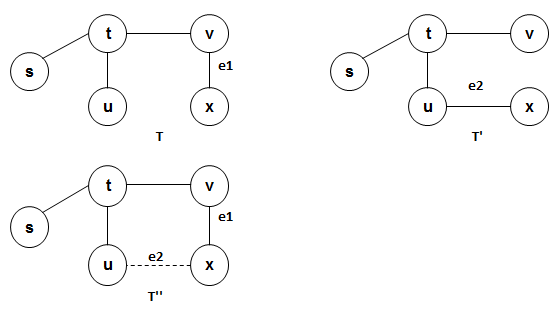
\includegraphics[width=0.8\textwidth]{q8-02.png}
\captionof{figure}{Exemplo de grafo com uma única MST com pesos nas arestas diferentes.}
\label{fig:8.2-1}
\end{center}